\section{PPO与Direct SAC协同求解}
\label{sec:algorithm}
\subsection{大时间尺度部署策略}
图\ref{fig:framework}展示了整体结构。部署策略使用大层观测，路由策略使用小层观测；两层之间通过实际位置、链路和任务队列发生联系，不额外传递一个未经执行的理想路由或理想服务能力。Direct SAC中的“Direct”仅表示策略直接产生路由分数，没有优化器教师、路由先验或残差修正模块；它不是在SAC之外重新命名一种未经验证的优化算法。

\begin{figure*}[t]
\centering
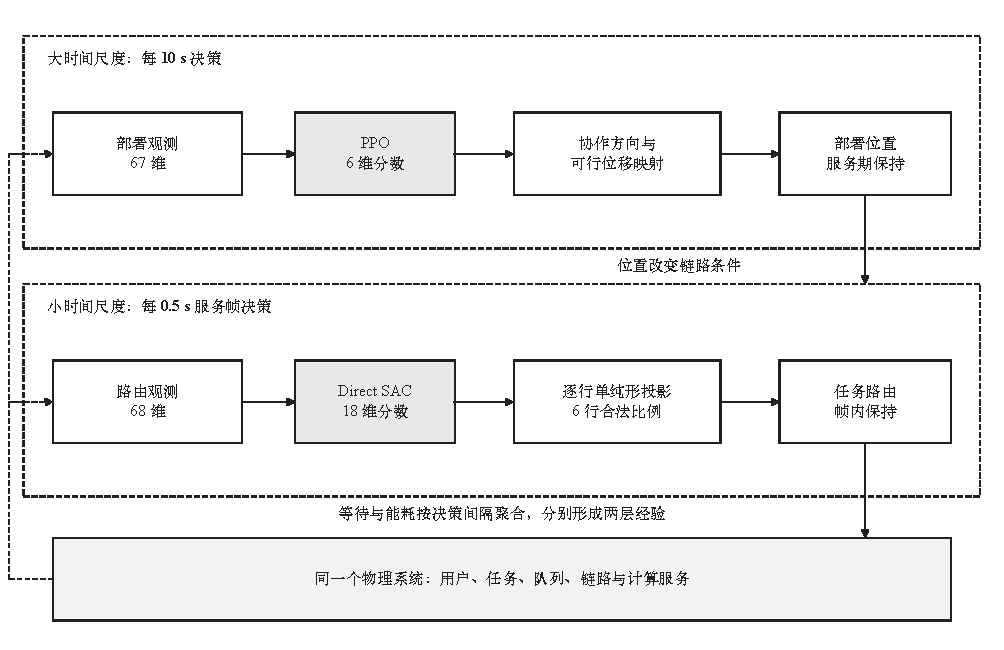
\includegraphics[width=\textwidth]{figures/fig4_framework.pdf}
\caption{PPO与Direct SAC协同框架：不同观测、不同决策频率及共同物理系统}
\label{fig:framework}
\end{figure*}

PPO策略参数记为$\theta$，其均值网络为$\vct\mu_\theta$。在部署观测$\vct o_t^{\mathrm L}$下，采样原始动作
\begin{equation}
 \vct a_t^{\mathrm L}\sim
 \mathcal N\!\left(\vct\mu_\theta(\vct o_t^{\mathrm L}),
 \diag(\vct\sigma_{\mathrm L}^2)\right).
 \label{eq:ppoaction}
\end{equation}
其中，$\vct\sigma_{\mathrm L}\in\R_{>0}^{2N}$为部署探索标准差，动作及标准差均为无量纲分数。将动作按节点分成$\vct a_{n,t}^{\mathrm L}\in\R^2$，先逐坐标限制至$[-1,1]$，再映射至单位圆盘：
\begin{equation}
 \begin{aligned}
 \widetilde{\vct a}_{n,t}&=\clip(\vct a_{n,t}^{\mathrm L},-1,1),\\
 \vct b_{n,t}&=\frac{\widetilde{\vct a}_{n,t}}
 {\max\{1,\|\widetilde{\vct a}_{n,t}\|_2\}}.
 \end{aligned}
 \label{eq:diskmap}
\end{equation}
$\clip$表示逐元素区间限制，$\vct b_{n,t}$为单位圆盘内的二维向量。它属于算法动作解码，不是用户移动或无线传播模型的一部分。

为使部署分数与当前负载空间关系对应，构造正交基$\mat B_n[t]\in\R^{2\times2}$。其第一列从本源群的业务质心指向协作参考无人机的当前位置，第二列与第一列垂直。当前负载最重的节点选择最轻节点为参考，其他节点选择最重节点为参考；两点重合时使用水平正方向及其垂直方向。该基只旋转动作坐标，不强制无人机向参考节点飞行。令$r_{\mathrm w}$为候选目标相对业务质心的半径，单位为m，则
\begin{equation}
 \vct y_n[t]=\Pi_{[0,L]^2}
 \big(\vct c_n[t]+r_{\mathrm w}\mat B_n[t]\vct b_{n,t}\big).
 \label{eq:waypoint}
\end{equation}
其中，$\vct y_n[t]\in\R^2$为候选目标，$\Pi_{[0,L]^2}$表示区域边界投影，$r_{\mathrm w}=60$ m。记$\vct q_n^{\mathrm b}[t]=\vct q_n[tJF]$为部署前位置，$\vct e_n[t]=\vct y_n[t]-\vct q_n^{\mathrm b}[t]$为候选目标偏移，$d_n^{\mathrm{tar}}[t]=\|\vct e_n[t]\|_2$为对应距离，二者单位为m。候选位移为
\begin{equation}
 \widetilde{\vct d}_n[t]=
 \frac{\min\{d_{\max},d_n^{\mathrm{tar}}[t]\}}
 {\max\{d_n^{\mathrm{tar}}[t],\epsilon_d\}}\vct e_n[t].
 \label{eq:displacement}
\end{equation}
$\epsilon_d>0$为仅防止零除的极小距离常数，单位为m。当候选距离不超过0.5 m时置零。随后，环境对全部候选位移执行联合路径安全修正，得到实际$\vct d_n[t]$。该修正可能进一步减少移动，不保证仍精确到达式\eqref{eq:waypoint}的候选位置。下层始终读取修正后实际位置形成的链路条件。

PPO的行为样本必须保留式\eqref{eq:ppoaction}的原始高斯分数及其对数概率，不能用裁剪后的物理动作重新代入高斯密度。令$\theta_{\mathrm{old}}$表示收集当前样本时的策略参数，重要性比率为
\begin{equation}
 \zeta_t(\theta)=
 \frac{\pi_\theta(\vct a_t^{\mathrm L}\mid\vct o_t^{\mathrm L})}
 {\pi_{\theta_{\mathrm{old}}}(\vct a_t^{\mathrm L}\mid\vct o_t^{\mathrm L})}.
 \label{eq:pporatio}
\end{equation}
分母在当前轮更新中固定。若在利用旧样本之前改变高斯标准差，会改变行为概率并破坏该比率的含义，因此探索标准差仅在当前采样缓冲清空之后调整。

大层价值网络记为$V_\psi$，参数为$\psi$。采用广义优势估计（generalized advantage estimation，GAE），定义
\begin{equation}
 \begin{aligned}
 \delta_t^{\mathrm V}&=R_t^{\mathrm L}
 +\Gamma_{\mathrm L}V_\psi(\vct o_{t+1}^{\mathrm L})
 -V_\psi(\vct o_t^{\mathrm L}),\\
 \widehat A_t&=\delta_t^{\mathrm V}
 \Gamma_{\mathrm L}\lambda_{\mathrm{GAE}}\xi_t\widehat A_{t+1}.
 \end{aligned}
 \label{eq:gae}
\end{equation}
其中，$\delta_t^{\mathrm V}$为时序差分残差，$\widehat A_t$为优势估计，$\lambda_{\mathrm{GAE}}\in[0,1]$为优势衰减系数；$\xi_t$指示采样序列是否在下一项继续，遇到采样流重置时取0。采样截断只切断第二行的递推，不把第一行的真实后继价值删除。

以$\overline A_t$表示当前样本批内标准化后的优势，$\epsilon_{\mathrm P}>0$为PPO裁剪范围，最大化
\begin{equation}
 \begin{aligned}
 \bar\zeta_t(\theta)&=\clip(\zeta_t(\theta),1-\epsilon_{\mathrm P},1+\epsilon_{\mathrm P}),\\
 L_{\mathrm P}(\theta)&=
 \E_t\!\left[\min\left\{\zeta_t(\theta)\overline A_t,\,
 \bar\zeta_t(\theta)\overline A_t\right\}\right].
 \end{aligned}
 \label{eq:ppoobjective}
\end{equation}
其中，$\bar\zeta_t(\theta)$为裁剪后的重要性比率。价值网络以$\widehat A_t+V_\psi(\vct o_t^{\mathrm L})$作为固定回归目标，更新时目标不参与梯度计算。训练还监测新旧策略的Kullback--Leibler（KL）散度近似，超过预设阈值时提前结束本轮策略迭代。裁剪和KL监测用于控制更新幅度，不能作为全局最优或单调性能改进的证明。

\subsection{小时间尺度路由与执行价值表征}
SAC策略参数记为$\phi$。演员网络输出均值$\vct\mu_\phi$和对数标准差，经重参数化得到
\begin{equation}
 \begin{aligned}
 \vct \epsilon&\sim\mathcal N(\vct0,\mat I),\\
 \vct u_s&=\vct\mu_\phi(\vct o_s^{\mathrm S})
 +\vct\sigma_\phi(\vct o_s^{\mathrm S})\odot\vct\epsilon,\\
 \vct z_s&=\tanh(\vct u_s).
 \end{aligned}
 \label{eq:sacaction}
\end{equation}
其中，$\vct u_s,\vct z_s,\vct\epsilon\in\R^{2N^2}$，$\mat I$为相应维数单位矩阵，$\odot$表示逐元素乘积。$\vct u_s$是未压缩高斯变量，$\vct z_s$是环境接收的有界原始分数，两者都不是路由概率。对数概率$\log\pi_\phi(\vct z_s\mid\vct o_s^{\mathrm S})$包含$\tanh$变换的雅可比修正，不含随后单纯形投影的概率密度变换。

将$\vct z_s$重排为$2N$个长度为$N$的行向量$\vct z_{i,p}$。每行独立求解标准欧氏单纯形投影\cite{duchi2008}：
\begin{equation}
 \begin{aligned}
 \vct\rho_{i,p}&=
 \argmin_{\vct r\in\Delta_N}\tfrac12\|\vct r-\vct z_{i,p}\|_2^2,\\
 \Delta_N&=\{\vct r\in\R^N:r_j\ge0,\ \sum_jr_j=1\}.
 \end{aligned}
 \label{eq:simplexprojection}
\end{equation}
其中，$\vct r$为该局部投影问题的辅助变量，$\Delta_N$为概率单纯形。该操作只将策略分数转换为合法动作，不使用队列代价求解额外路由优化，也不构成逐次凸近似教师。

为计算投影，将本行分数降序排列为$z_{(1)}\ge\cdots\ge z_{(N)}$，定义
\begin{equation}
 \begin{aligned}
 k^\star&=\max\left\{k:\
 z_{(k)}-\frac{\sum_{j=1}^{k}z_{(j)}-1}{k}>0\right\},\\
 \vartheta&=\frac{\sum_{j=1}^{k^\star}z_{(j)}-1}{k^\star},\qquad
 \rho_j=\max\{z_j-\vartheta,0\}.
 \end{aligned}
 \label{eq:projectionclosed}
\end{equation}
这里$k^\star$为正支撑项数，$\vartheta$为该行投影阈值，$\rho_j$为恢复原列顺序后的目的比例；求和内的$k,j$是本行排序位置，不表示用户与无人机物理编号。浮点运算后可按行再归一化以消除舍入误差。算法\ref{alg:route}列出了执行步骤。

\begin{algorithm}[t]
\caption{Direct SAC路由动作解码}
\label{alg:route}
\small
\begin{algorithmic}[1]
\Require 当前小层观测$\vct o^{\mathrm S}$，策略$\pi_\phi$，节点数$N$
\Ensure 原始分数$\vct z$、合法执行路由$\vct\rho$
\State 按式\eqref{eq:sacaction}采样$\vct z$并计算分数对数概率
\State 将$\vct z$重排为$2N$行、每行$N$列
\For{每个优先级$p$与源节点$i$}
  \State 对行分数降序排序，计算各前缀和
  \State 按式\eqref{eq:projectionclosed}确定$k^\star$与$\vartheta$
  \State 按原列顺序求$\rho_{ij,p}=\max\{z_{ij,p}-\vartheta,0\}$
  \State 用行和校正浮点误差，保留零比例
\EndFor
\State 在本服务帧内保持$\vct\rho$，仅作用于新待拆分任务
\State 同时保留$\vct z$与$\vct\rho$供回放及动作核验
\end{algorithmic}
\end{algorithm}

对于$N=3$，演员输出18维分数，执行路由也是18个数，但6行各有一个和为1的约束，物理路由的自由度为$2N(N-1)=12$。因此，不能将“12个独立自由度”写成“演员实际输出12维动作”。欧氏投影允许精确零分配和全本地处理，同时存在多对一映射，多个不同分数可产生完全相同的执行路由。

图\ref{fig:sac}区分了分数空间和执行空间。双评论家参数记为$\omega_1,\omega_2$，采用
\begin{equation}
 Q_{\omega_\ell}(\vct o,\vct z)
 =q_{\omega_\ell}\big(\vct o,\mathcal P_\Delta(\vct z)\big),
 \qquad \ell\in\{1,2\}.
 \label{eq:executedcritic}
\end{equation}
其中，$q_{\omega_\ell}$的动作输入为执行路由，$\ell$索引两个评论家，$\vct o$为小层观测的简写。在线网络与目标网络使用相同投影。若两个分数映射到相同路由，式\eqref{eq:executedcritic}使其获得相同的当前价值输出，避免评论家仅因无物理差异的分数表示而给出不同估值。

\begin{figure*}[t]
\centering
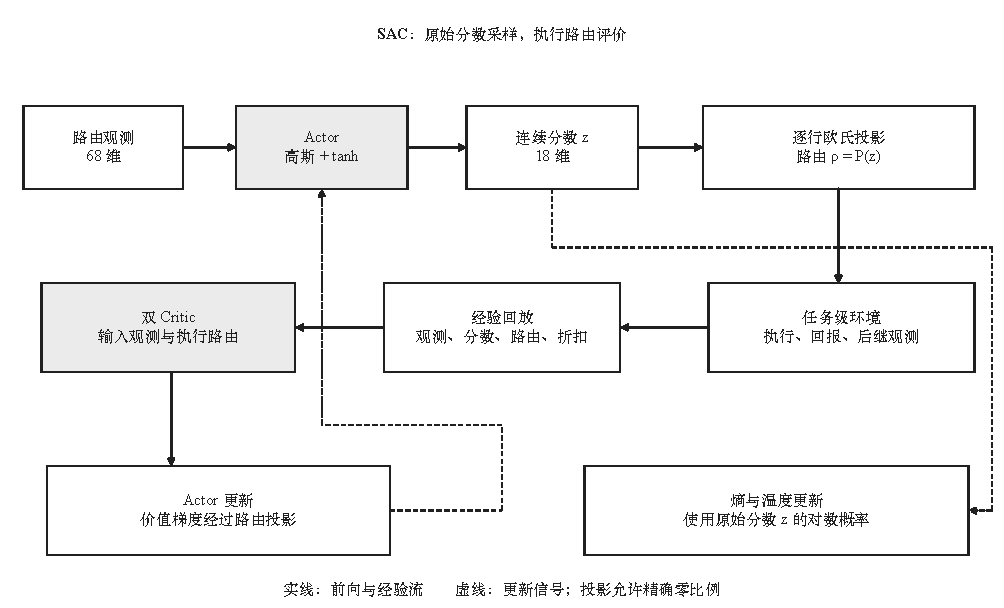
\includegraphics[width=\textwidth]{figures/fig5_sac.pdf}
\caption{SAC采样与更新：评论家评价执行路由，熵项仍在原始分数空间计算}
\label{fig:sac}
\end{figure*}

从回放缓冲$\mathcal D$采样经验，令$\vct o'$为真实后继观测，$\vct z'\sim\pi_\phi(\cdot\mid\vct o')$，$\bar\omega_1,\bar\omega_2$为目标评论家参数，$\alpha>0$为熵温度。时序差分目标为
\begin{equation}
 \begin{aligned}
 y={}&\widehat r+\widehat\gamma\left[
 \min_{\ell=1,2}q_{\bar\omega_\ell}
 \big(\vct o',\mathcal P_\Delta(\vct z')\big)\right.\\
 &\left.\hspace{18mm}-\alpha\log\pi_\phi(\vct z'\mid\vct o')\right].
 \end{aligned}
 \label{eq:sactarget}
\end{equation}
$\widehat r$与$\widehat\gamma$逐条取自经验，按式\eqref{eq:boundary}区分普通与跨部署样本。目标构造不传播梯度，评论家最小化
\begin{equation}
 L_Q=\E_{\mathcal D}
 \sum_{\ell=1}^2
 \left[q_{\omega_\ell}(\vct o,\mathcal P_\Delta(\vct z))-y\right]^2.
 \label{eq:criticloss}
\end{equation}
演员使用当前观测重新采样分数，最小化
\begin{equation}
 \begin{aligned}
 L_\pi=\E_{\vct o\sim\mathcal D,\vct z\sim\pi_\phi}
 \left[\vphantom{\min_{\ell=1,2}}\right.&\alpha\log\pi_\phi(\vct z\mid\vct o)\\
 &\left.-\min_{\ell=1,2}q_{\omega_\ell}
 (\vct o,\mathcal P_\Delta(\vct z))\right].
 \end{aligned}
 \label{eq:actorloss}
\end{equation}
更新演员时固定评论家参数，但允许价值梯度经过执行路由与可微投影返回演员。若只在环境执行时投影而在价值更新时仍输入不受约束的分数，将不再是式\eqref{eq:executedcritic}所规定的执行路由表征。

温度按自动熵调节方式更新\cite{sacapplications2018}。令$\beta=\ln\alpha$为待优化标量，$\mathcal H_{\mathrm{tar}}=-2N^2=-18$为分数空间目标熵，采用损失
\begin{equation}
 L_\alpha=-\E\!\left[
 \beta\big(\log\pi_\phi(\vct z\mid\vct o)+\mathcal H_{\mathrm{tar}}\big)
 \right].
 \label{eq:alphaloss}
\end{equation}
括号中的采样对数概率在温度更新时停止梯度。由于$\mathcal P_\Delta$多对一且可将连续分数映射至低维面或顶点，本文不将该熵解释为执行路由的微分熵，也不把执行自由度12代入声称已经优化12维路由密度。执行价值表征减少的是评论家对等价分数的区分，尚不能消除策略在冗余分数方向探索的可能性。

\subsection{训练流程与边界处理}
两层采用先小层预训练、后联合训练的流程。预训练阶段PPO不更新，其原始部署分数置零。由式\eqref{eq:waypoint}可知，此时无人机仍按业务质心形成候选目标并受实际位移与安全约束控制，所以这是动态质心部署，不是无人机位置完全固定。SAC在该部署规则下学习路由，为联合训练提供当前场景产生的初始参数与回放经验。联合阶段继续保留小层优化器和经验，开始采集、更新PPO，禁止把历史不同观测维数或不同奖励训练得到的权重直接作为当前结果。

演员、评论家均采用两层隐藏网络，每层256个单元。两层输入维数分别由式\eqref{eq:microdim}、式\eqref{eq:macrodim}决定，而不通过补零伪装相同观测。SAC回放容量为$10^5$条，批大小为128，积累至少1000条经验后开始学习，每20个服务帧更新一次评论家；每个阶段开始的前100次评论家更新不更新演员，之后每两次评论家更新一次演员。该延迟只用于学习时序，执行策略仍在每个服务帧产生动作。

SAC预训练阶段的演员、评论家和温度学习率分别为$3\times10^{-5}$、$3\times10^{-4}$和$3\times10^{-5}$，联合阶段分别为$3\times10^{-5}$、$10^{-4}$和$10^{-5}$。目标网络使用系数0.01进行软更新。PPO每累计300个大周期样本执行一次更新，策略与价值学习率分别为$3\times10^{-4}$和$10^{-3}$，至多执行10轮策略更新，裁剪范围为0.2，KL阈值为0.03，GAE系数为0.95。各网络梯度范数上限设为1，以限制单次数值更新，而不修改物理奖励定义。

算法\ref{alg:joint}给出完整采样逻辑。关键不是简单交替调用两种算法，而是使动作、回报和后继观测对应同一段真实时间。周期末的小层经验先暂存，待下一次部署结束后再补齐回报与后继；日志输出不触发环境重置。PPO原始动作与行为对数概率成对存储，标准差调度不修改已有样本的行为策略。

\begin{algorithm*}[t]
\caption{具有真实部署边界的双时间尺度训练}
\label{alg:joint}
\small
\begin{algorithmic}[1]
\Require 场景配置、两层观测映射、物理代价、预训练及联合预算
\Ensure 当前配置下的SAC与PPO参数，配套训练及评估记录
\State 初始化网络、目标网络、SAC回放$\mathcal D$与PPO采样缓冲；不载入旧场景权重
\For{预训练阶段及随后获准开展的联合阶段}
 \For{每条连续采样流}
  \State 重置场景一次；设置周期末待补经验为空
  \For{流内每个大周期$t$}
   \State 读取$\vct o_t^{\mathrm L}$；预训练取零分数，联合阶段按PPO采样原始动作及对数概率
   \State 解码并安全修正部署位移；执行两个部署帧，记录真实回报
   \State 生成首个服务帧的当前到达并提取小层观测
   \State 若存在上一周期待补经验，按式\eqref{eq:boundary}补齐并写入$\mathcal D$
   \For{当前周期的18个服务帧}
    \State 用算法\ref{alg:route}产生路由；执行5个物理步并累计式\eqref{eq:framereward}的回报
    \State 普通帧读取下一服务观测并存经验；末服务帧暂存，等待下一部署结束
    \State 满足更新间隔及暖启动条件时，按式\eqref{eq:sactarget}--\eqref{eq:alphaloss}更新SAC
   \EndFor
   \State 汇总式\eqref{eq:macroreward}的周期回报，推进业务阶段，读取真实大层后继观测
   \State 联合阶段存PPO样本；样本充足时按式\eqref{eq:gae}--\eqref{eq:ppoobjective}更新
   \State 到300 s统计边界时只输出日志，不清除任务与队列
  \EndFor
  \State 采样截断处在重置前执行下一部署，补全最后一条SAC经验
  \State 大层保留真实后继价值，停止跨场景的GAE递推
 \EndFor
 \State 按预先声明的验证协议核验阶段质量，记录是否实际进入联合阶段
\EndFor
\end{algorithmic}
\end{algorithm*}

预训练预算与是否进入联合阶段必须随实验记录一同报告。配置中存在联合训练轮数，不等于PPO已经更新；同样，接口冒烟测试发生过一次PPO更新，也不能替代完整联合训练。预算调整应作为独立实验设置记录，不回写已完成结果。本文将训练机制与最终实验结论分开陈述，以便在新一轮训练完成后直接填入相应结果而不改变前述模型口径。

\subsection{动作性质与复杂度分析}
单纯形投影具有明确的可行性性质。式\eqref{eq:simplexprojection}的目标严格凸、可行域非空闭凸，因此每行投影存在唯一解。其最优性条件给出$\rho_j=\max\{z_j-\vartheta,0\}$，选择式\eqref{eq:projectionclosed}的阈值后行和为1，故任意有限分数均可转换为满足式\eqref{eq:simplexconstraint}的路由。进一步，对任意$\vct r\in\Delta_N$，取$\vct z=\vct r-\frac12\vct1$，则所有分数位于$[-\frac12,\frac12]$，且$\mathcal P_\Delta(\vct z)=\vct r$。其中，$\vct1$为全1向量。因此，有界分数加投影不排除任何合法路由，包括单节点顶点动作。

当一行投影的正支撑集合$\mathcal S=\{j:\rho_j>0\}$在局部保持不变时，其雅可比元素为
\begin{equation}
 \frac{\partial\rho_j}{\partial z_k}=
 \begin{cases}
 \ind{j=k}-1/|\mathcal S|,&j,k\in\mathcal S,\\
 0,&\text{其他}.
 \end{cases}
 \label{eq:jacobian}
\end{equation}
$\ind{j=k}$为指示函数，条件成立取1，否则取0。该表达式说明投影在固定支撑区域内可微，而在支撑改变的分界处仅分段可微。数值实现通过自动微分给出所采用分支的梯度，不能将其解释为所有边界上均存在唯一普通导数。尤其在顶点对应的局部区域，价值梯度可能对部分分数方向为零；动作可行性不保证探索一定充分。

执行价值表征的性质也应与收敛性质区分。给定相同完整物理状态，若$\mathcal P_\Delta(\vct z_1)=\mathcal P_\Delta(\vct z_2)$，则当前任务分配、即时物理代价和条件物理转移相同。式\eqref{eq:executedcritic}显式满足这种分数等价性。然而，聚合观测可能对应多个完整状态，两层联训还带来策略变化；因此，满足分数等价性不意味着消除了部分可观测性、离策略误差或函数逼近误差。

下面分析控制计算量，不将通信传输时间混入CPU算法运行时间。设隐藏宽度为$W$，小层动作维数为$d_a=2N^2$。两层隐藏的全连接演员单次前向计算量为$\mathcal O(d_{\mathrm S}W+W^2+Wd_a)$。逐行排序投影处理$2N$行，每行排序复杂度为$\mathcal O(N\log N)$，因此小层单次决策为
\begin{equation}
 \mathcal O\!\left(d_{\mathrm S}W+W^2+Wd_a+N^2\log N\right).
 \label{eq:microcomplexity}
\end{equation}
这里$\mathcal O(\cdot)$表示渐近运算量。$N=3$时排序规模很小，但不能据此将训练网络的代价忽略。大层演员的前向量为$\mathcal O(d_{\mathrm L}W+W^2+WN)$，动作坐标变换为$\mathcal O(N)$，两两距离与安全检查至少涉及$\mathcal O(N^2)$关系；若安全修正执行$K_{\mathrm{safe}}$轮两两检查，则该部分为$\mathcal O(K_{\mathrm{safe}}N^2)$。

设训练批大小为$B_{\mathrm{tr}}$，小层一次双评论家及演员更新的主导量为
\begin{equation}
 \mathcal O\!\left(
 B_{\mathrm{tr}}\big[(d_{\mathrm S}+d_a)W+W^2+N^2\log N\big]
 \right).
 \label{eq:traincomplexity}
\end{equation}
双网络、目标网络与多次反向传播改变常数因子。若PPO批量含$B_{\mathrm P}$个周期、更新$K_{\mathrm P}$轮，则其主导量为$\mathcal O(K_{\mathrm P}B_{\mathrm P}[(d_{\mathrm L}+2N)W+W^2])$。设回放容量为$M_{\mathrm R}$，同时保存两端观测、原始分数、执行路由、回报和后继折扣，存储量为$\mathcal O(M_{\mathrm R}(2d_{\mathrm S}+2d_a+2))$。

仿真环境本身还需处理用户和任务。设物理步$m$保留的父任务记录数为$P_m$，该步扫描或完成处理的分片数为$C_m$，则任务统计与队列服务开销还包含$\mathcal O(K+N^2+P_m+C_m)$，不能把神经网络前向时间当作整个系统步进时间。正式报告应在指定硬件下分别测量控制器推理、动作映射和环境仿真耗时。上述性质只说明可行性、表征一致性和运算规模，不构成两层深度强化学习全局收敛证明。
